\toclesssection{SCP 015 - Pipe Nightmare}
\addcontentsline{toc}{section}{SCP 015 - Pipe Nightmare}

\textbf{Item \#:} SCP-015

\textbf{Object Class:} Euclid

\begin{figure}[h]
\begin{center}
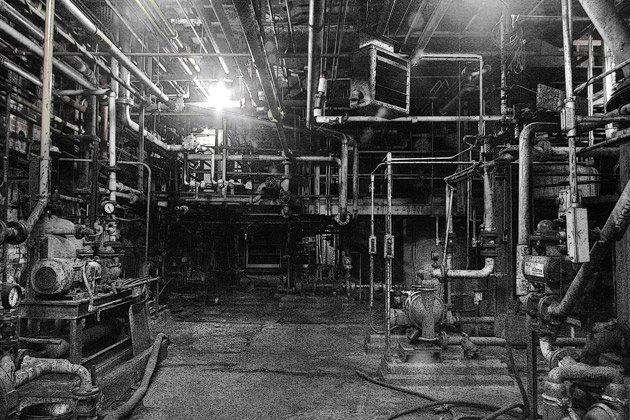
\includegraphics[scale=0.4]{scp/015.jpg}
\linebreak SCP-015
\end{center}
\end{figure}

\textbf{Special Containment Procedures:} SCP-015 is impossible to move, and is contained on-site. A gap of at least 2 m (6 ft) needs to be maintained around the entire structure containing SCP-015 at all times, and no structures of any kind are to make contact with SCP-015's current containment structure. Exploration is permissible, but only in teams of three (3) with full safety lines and GPS tracking. Any protrusions from SCP-015 must be capped and sealed immediately, with the new site recorded and logged.

No aggressive action is to be made within SCP-015. No hand or power tools are allowed anywhere inside SCP-015. No repairs or maintenance are to be made anywhere on SCP-015.

\textbf{Description:} SCP-015 is a mass of pipes, vents, boilers and other various plumbing apparatus completely filling a warehouse in \censor{XXXXXXX}. The pipes appear to grow when not under observation, attempting to connect to nearby structures via sewer systems and underground plumbing. SCP-015 contains, at current estimate, over 190 kilometers (120 miles) of pipes, ranging in diameter from 2.5 cm to over 1 m. Some pipes appear new, while others are rusted and leaking. Pipes have been reported as being made of bone, wood, steel, pressed ash, human flesh, glass, and granite. No pipes composed of lead, PVC plastic, copper, or any other traditional material for the production of pipes have been found.

SCP-015 reacts to tools and aggression. Any personnel acting violently, carrying tools, or attempting to damage or repair SCP-015 in any way, will trigger a reaction. Any pipes near the subject will burst, spraying on the subject for several seconds before the flow suddenly stops. Pipes have been reported containing oil, mercury, rats, a species of insect not yet identified, ground glass, sea water, entrails, and molten iron. Pipes will continue to burst around subject until death or retreat.

SCP-015 was cut back to its current structure after attaching to 11 other structures in the area. Currently, 11 personnel have been killed, and 20 more are still missing. Reports have been made of banging and screaming coming from within SCP-015.